\section{Looking at the backreflex}
We now placed the PD on the backreflecting light beam. So now, we expect to see dips instead of peaks in our signal.


\begin{figure}[htbp]
    \centering
    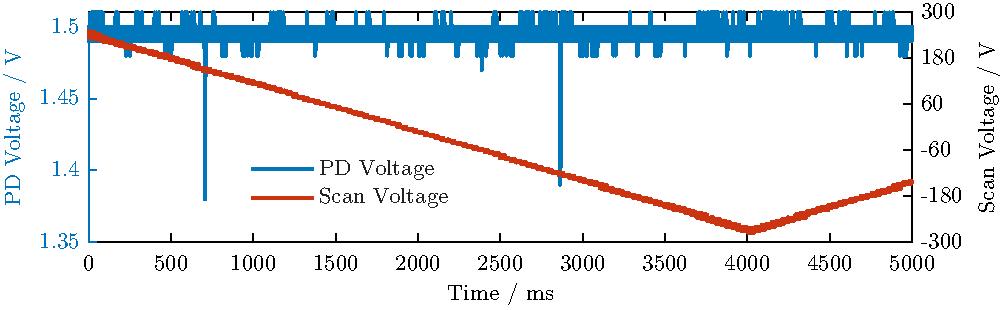
\includegraphics[width=\textwidth]{back/Figure_1.pdf}
    \caption{Here, we see dips instead of peaks. However, it appears that more peaks are visible in the backreflecting beam than in the transmitted beam. In the transmitted beam, only two peaks were prominently visible. The signal also is much more noisy.}
\end{figure}
Now, I inverted the signal in order to be able to use my existing code for further analysis. I kept the EOM running to compare the FHWM.

\begin{figure}[htbp]
    \centering
    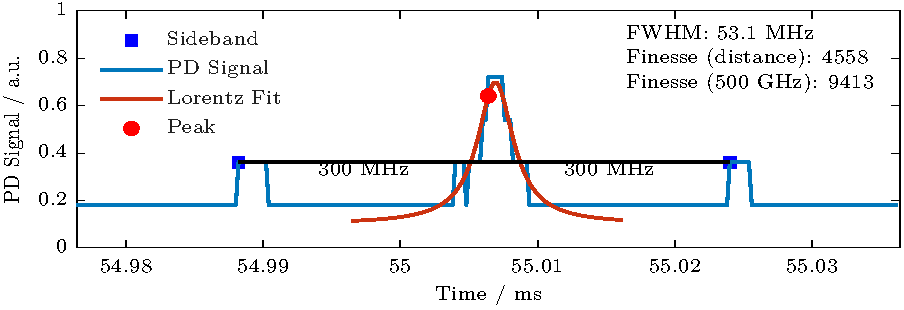
\includegraphics[width=\textwidth]{back/Figure_6.pdf}
    \caption{Zoomed in on one peak with its sidebands.}
\end{figure}
\begin{figure}[htbp]
    \centering
    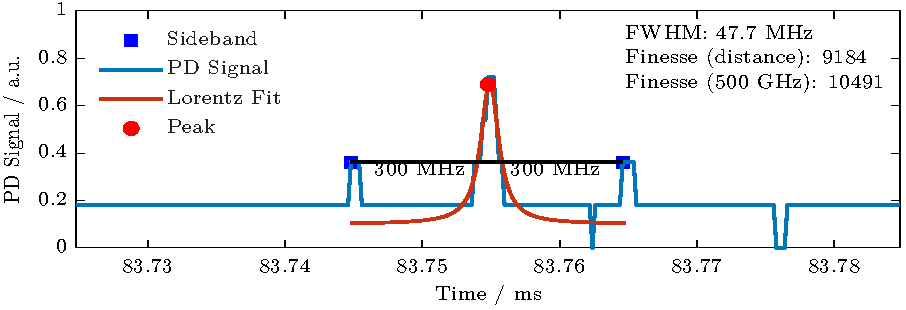
\includegraphics[width=\textwidth]{back/Figure_8.pdf}
    \caption{Zoomed in on antoher peak with its sidebands.}
\end{figure}

The FWHM values seem to be larger than in the transmission setup. However, the fit also looks fairly poor so I would take these results with a grain of salt.
